\chapter{Testing}
\label{chap:testing}

\section{Testing for Correctness of Functionality}
As the library is built on other crates, the only tests which can be performed are those on individual components of the protocol, and full run-throughs of the entire protocol.

\subsection{Testing Individual Components}
Traditionally in cryptographic software, test-vectors have been used to test for the correct functionality of various componenets.
However due to the use of Ristretto255, instead of raw Curve25519, there are no test-vectors available.
Once the implementation was feature complete, I emailed Bj\"orn Haase to discuss test vector creation\footnote{Bj\"orn is the creator of AuCPace}.
He was interested in the project and mentioned they were interested in a second implementation of \gls{aucpace} at Endress+Hauser.
However he did not have the time to create test vectors and by this point in the project I was too busy to do so as well.
So while test vectors have not yet been created, it is likely they will be in the near future.

\subsection{Integration Testing}
To perform integration testing, the tests were split into four categories based on which of the two major features they required\footnote{This work was completed after the code freeze, so is only available on the github.}.

\begin{center}
  \rowcolors{0}{}{mintbg}
  \captionof{table}{Integration Tests Split}
  \label{tab:aucpace-int-tests}
  \begin{tabularx}{\linewidth}{ ccX }
    \toprule
    \texttt{strong\_aucpace} & \texttt{partial\_aug} & test \\
    \midrule
    \xmark & \xmark & \texttt{test\_key\_agreement.rs} \\
    \xmark & \cmark & \texttt{test\_key\_agreement\_partial\_aug.rs} \\
    \cmark & \xmark & \texttt{test\_key\_agreement\_strong.rs} \\
    \cmark & \cmark & \texttt{test\_key\_agreement\_strong\_partial\_aug.rs} \\
    \bottomrule
  \end{tabularx}
\end{center}

Inside of each test file there are two main scaffolding functions: \texttt{init} and \texttt{test\_core}, the former Perfoms the initial setup of the client, server and database, and the latter performs all the functionality which is common to every test.
From there there are four tests in each file, each testing the following:

\begin{center}
  \rowcolors{0}{}{mintbg}
  \captionof{table}{Per-file Test Splits}
  \label{tab:aucpace-int-tests-file}
  \begin{tabularx}{\linewidth}{ ccX }
    \toprule
    \texttt{static SSID} & \texttt{implicit auth} & test \\
    \midrule
    \xmark & \xmark & \texttt{test\_key\_agreement} \\
    \xmark & \cmark & \texttt{test\_key\_agreement\_implicit\_auth} \\
    \cmark & \xmark & \texttt{test\_key\_agreement\_prestablished\_ssid} \\
    \cmark & \cmark & \texttt{test\_key\_agreement\_prestablished\_ssid\_implicit} \newline \texttt{\_auth} \\
    \bottomrule
  \end{tabularx}
\end{center}

\section{The Ultimate Test}
As with any piece of software the ultimate test is to get the entire thing running / working on real hardware.

\subsection{Choosing the Microcontroller / Platform}
Because \gls{aucpace} is intended for use in the \gls{iiot}, it was decided that an \gls{stm} based \gls{mcu} would be a good fit.
\gls{stm} \glspl{mcu} are very prevelant in industry, have many dev boards supporting a wide variety of different chips, and they also have excellent Rust support.
Following this decision the NUCLEO-F401RE dev board was selected.
It is a small \gls{mcu} with a modest 512K of flash memory.
While certainly not the least powerful platform around it should be representative of a majority of \gls{iot} systems.

\begin{figure}[H]
  \centering

  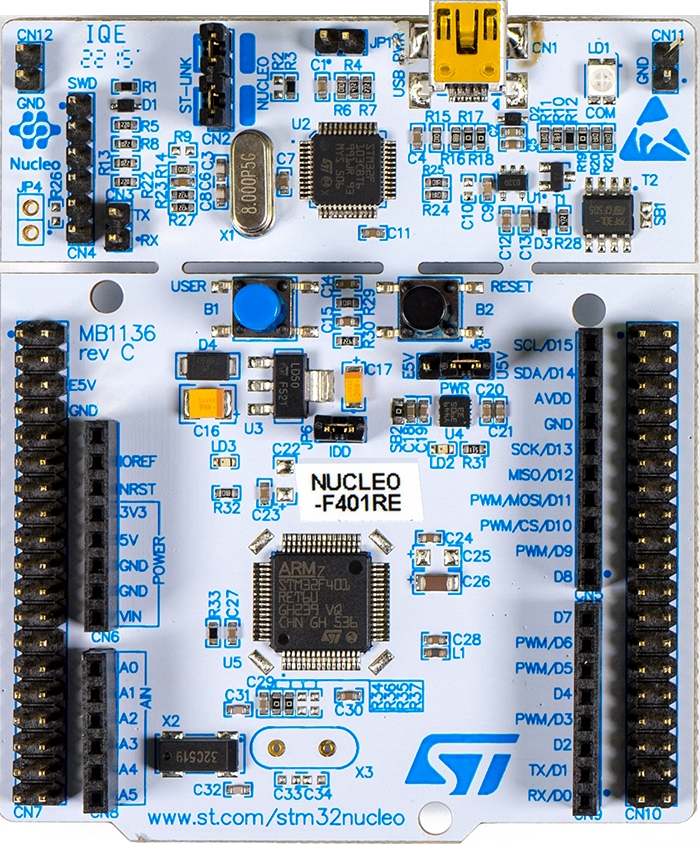
\includegraphics[angle=90,width=0.8\linewidth]{assets/stm32-f410re.jpg}
  \caption{NUCLEO-F401RE Dev Board}
  \label{fig:nucleo-f401re}
\end{figure}

\subsection{Choosing an Embedded Rust Platform}
Initially the \gls{rtic} framework was selected as example code for interacting over serial was easy to find online.
However getting \gls{rtic} to work on the actual board proved challenging as low level details such as clocks and timers confused things considerably.

After a few attempts\footnote{several days of work} with \gls{rtic}, efforts were switched to using the Embassy project.
This proved to greatly alleviate the strain of working in the embedded software world.
Embassy performs all low level setup for you and allows the programmer to work with async/await constructs instead of timers etc.
There was still some considerable strife in getting the serial connection to work consistently.
After a lengthy conversation with \texttt{sjm\#0205} on the Rust discord server, we came to the conclusion that the board's low quality crystal oscillators were causing the serial connection to get out of sync.
Reducing the baud rate to 28800 resulted in a much more reliable connection, this is due to clock accuracy being less important at lower baud rates as there is a bigger margin for error in when lines go high/low\footnote{This solution was found after code freeze so is only available on the github}.
After establishing a reliable serial connection work could now begin on implementing \gls{aucpace}.

\subsection{Implementing the AuCPace Protocol}
The server side of \texttt{examples/key\_agreement.rs} was initially adapted to fit the code structure of the embedded app.
However this immediately brought around a problem with the \gls{aucpace} implementation, it was refusing to compile.
As it happened this was a quirk of how Rust works that I wasn't aware of.
Care was taken to develop the library using the \verb|#![no_std]| attribute, this tells the compiler that this code isn't allowed to use the Rust standard library.
Even the \texttt{examples/key\_agreement\_no\_std.rs} example program wasn't enough to weed this out.
Because the standard library is still available when linking on x86, the \verb|#![no_std]| example still compiles, despite containing code from the standard library.
When it was adapted for the microcontroller, it was targeting \texttt{thumbv7em-none-eabihf}, the standard library is simply not available for this target as it doesn't have an operating system.
The malignant crate turned out to be \texttt{serde-arrays} which, although not containing any code that should require the standard library, it was not marked as \verb|#![no_std]| and thus fails to compile as it implicitly links to the standard library.
The solution was very simple thankfully, just weeks prior to attmpting this embedded example, a new crate was released \texttt{serde-byte-arrays}, this solved my problem better than \texttt{serde-arrays}, was marked \verb|#![no_std]| and was more efficient at the same time!
Once these two primitives were reliable, it was quite straightforward to implement the protocol in full.

\subsection{Benchmarking}
Benchmarking was performed by switching feature flags on and off on both the client and server.
An additional element of the compiler flags was added because Rust's compiler allows you to make tradeoffs between code-size and speed quite easily.
The easiest method for doing this is by creating a profile for the Rust compiler to use, there are two profiles normally available -- \texttt{debug} and \texttt{release}; \texttt{debug} is intended to be used during development and is tuned for fast compile times and extensive debug info. \texttt{release} is tuned for speed and removes all debug info normally.
In listing \ref{server-profile} the debug information is re-enabled for \texttt{release} mode, this means that the Rust compiler includes \gls{dwarf} debug infomation in the compiled binary.
A \texttt{server} profile is also listed, this profile inherits from \texttt{release} meaning that initially it is the same as \texttt{release}, \texttt{opt-level} is then set to \texttt{\enquote{s}}, this makes the compiler instead optimise for code size instead of speed.
The two remaining options -- \texttt{lto} and \texttt{codegen-units} are less significant and are just there to improve the information available to the compiler to allow it to generate more efficient code.

The \enquote{Compute time} was based on the compute time calculated by the server as it ran through the protocol as can be seen in \cref{fig:aucpace-embedded-server}.
These are based on just one measurement of the time, this is due to the use of constant time algorithms wherever possible, when the number of ticks was measured directly, the variance was on the order of 5 ticks, which is just 0.005ms ($5\mu$s), this variance is not big enough to effect the results.

\Cref{tab:aucpace-embedded-benchmarks-server,tab:aucpace-embedded-benchmarks-server-static,tab:aucpace-embedded-benchmarks-release,tab:aucpace-embedded-benchmarks-release-static} show the code size, compute time and the amount of data sent for each of the protocol variants supported via feature flags, each table is then split by compiler mode and whether a static SSID was used.
\Cref{fig:feature-effects} then shows a comparison of the effect of each of these variables.

\medskip

\tomlcode[label=server-profile]{Server Compiler Profile}{assets/server.toml}

\begin{figure}[H]
  \centering

  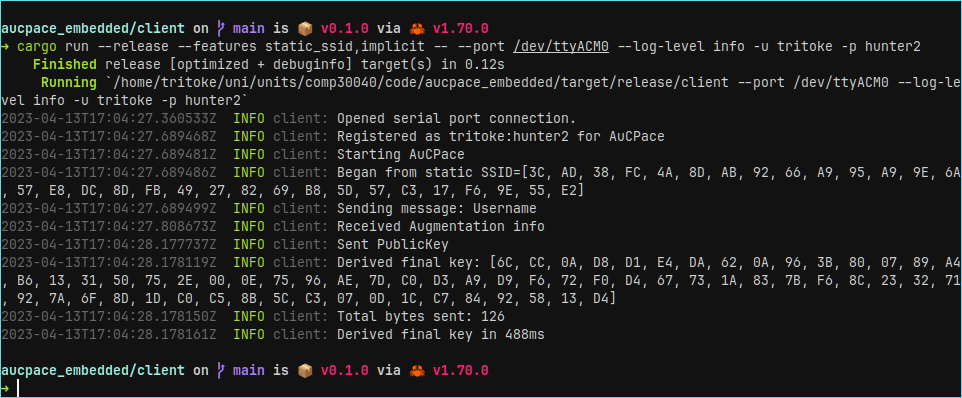
\includegraphics[width=\linewidth]{aucpace_embedded_client.png}
  \caption{AuCPace Embedded Client Output}
  \label{fig:aucpace-embedded-client}
\end{figure}

\begin{figure}[H]
  \centering

  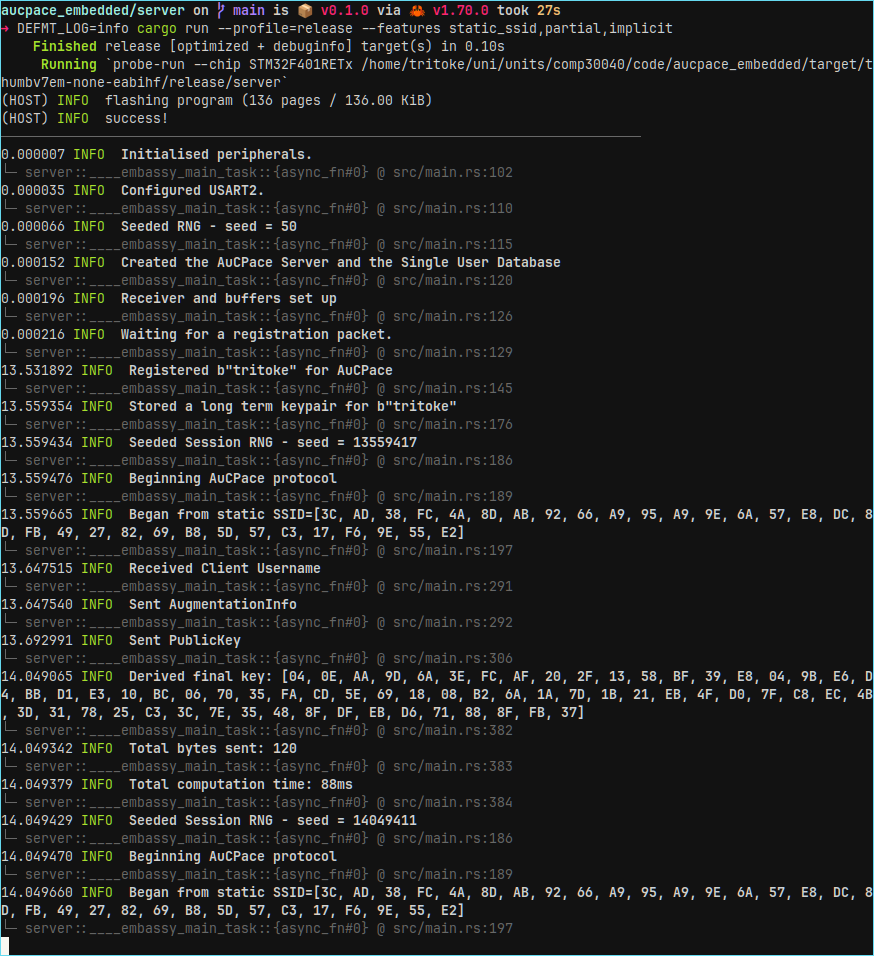
\includegraphics[width=\linewidth]{aucpace_embedded_server.png}
  \caption{AuCPace Embedded Server Output}
  \label{fig:aucpace-embedded-server}
\end{figure}

\begin{center}
  \small
  \rowcolors{0}{}{mintbg}
  \captionof{table}{Code size and compute time by feature flag with \texttt{profile=server}}
  \label{tab:aucpace-embedded-benchmarks-server}
  \begin{tabular}{ cccccc }
    \toprule
    \texttt{strong} & \texttt{implicit} & \texttt{partial} & code size (Kib) & compute time (ms) & data sent (bytes) \\
    \midrule
    \xmark & \xmark & \xmark & 82 & 171 & 342 \\
    \xmark & \xmark & \cmark & 83 & 139 & 342 \\
    \xmark & \cmark & \xmark & 83 & 134 & 206 \\
    \xmark & \cmark & \cmark & 83 & 103 & 206 \\
    \cmark & \xmark & \xmark & 88 & 171 & 383 \\
    \cmark & \xmark & \cmark & 88 & 139 & 383 \\
    \cmark & \cmark & \xmark & 87 & 135 & 247 \\
    \cmark & \cmark & \cmark & 88 & 103 & 247 \\
    \bottomrule
  \end{tabular}
\end{center}

\begin{center}
  \small
  \rowcolors{0}{}{mintbg}
  \captionof{table}{Code size and compute time by feature flag with \texttt{profile=server} and a static SSID}
  \label{tab:aucpace-embedded-benchmarks-server-static}
  \begin{tabular}{ cccccc }
    \toprule
    \texttt{strong} & \texttt{implicit} & \texttt{partial} & code size (Kib) & compute time (ms) & data sent (bytes) \\
    \midrule
    \xmark & \xmark & \xmark & 81 & 171 & 302 \\
    \xmark & \xmark & \cmark & 82 & 139 & 302 \\
    \xmark & \cmark & \xmark & 82 & 135 & 166 \\
    \xmark & \cmark & \cmark & 82 & 103 & 166 \\
    \cmark & \xmark & \xmark & 86 & 170 & 343 \\
    \cmark & \xmark & \cmark & 87 & 138 & 343 \\
    \cmark & \cmark & \xmark & 87 & 135 & 207 \\
    \cmark & \cmark & \cmark & 87 & 103 & 207 \\
    \bottomrule
  \end{tabular}
\end{center}

\begin{center}
  \small
  \rowcolors{0}{}{mintbg}
  \captionof{table}{Code size and compute time by feature flag with \texttt{profile=release}}
  \label{tab:aucpace-embedded-benchmarks-release}
  \begin{tabular}{ cccccc }
    \toprule
    \texttt{strong} & \texttt{implicit} & \texttt{partial} & code size (Kib) & compute time (ms) & data sent (bytes) \\
    \midrule
    \xmark & \xmark & \xmark & 132 & 148 & 342 \\
    \xmark & \xmark & \cmark & 137 & 119 & 342 \\
    \xmark & \cmark & \xmark & 132 & 117 & 206 \\
    \xmark & \cmark & \cmark & 138 & 90  & 206 \\
    \cmark & \xmark & \xmark & 139 & 148 & 383 \\
    \cmark & \xmark & \cmark & 142 & 120 & 383 \\
    \cmark & \cmark & \xmark & 139 & 116 & 247 \\
    \cmark & \cmark & \cmark & 142 & 89  & 247 \\
    \bottomrule
  \end{tabular}
\end{center}

\begin{center}
  \small
  \rowcolors{0}{}{mintbg}
  \captionof{table}{Code size and compute time by feature flag with \texttt{profile=release} and a static SSID}
  \label{tab:aucpace-embedded-benchmarks-release-static}
  \begin{tabular}{ cccccc }
    \toprule
    \texttt{strong} & \texttt{implicit} & \texttt{partial} & code size (Kib) & compute time (ms) & data sent (bytes) \\
    \midrule
    \xmark & \xmark & \xmark & 131 & 145 & 302 \\
    \xmark & \xmark & \cmark & 136 & 120 & 302 \\
    \xmark & \cmark & \xmark & 132 & 115 & 166 \\
    \xmark & \cmark & \cmark & 137 & 88  & 166 \\
    \cmark & \xmark & \xmark & 138 & 148 & 343 \\
    \cmark & \xmark & \cmark & 141 & 120 & 343 \\
    \cmark & \cmark & \xmark & 138 & 116 & 207 \\
    \cmark & \cmark & \cmark & 142 & 89  & 207 \\
    \bottomrule
  \end{tabular}
\end{center}

\begin{figure}[H]
  \centering
  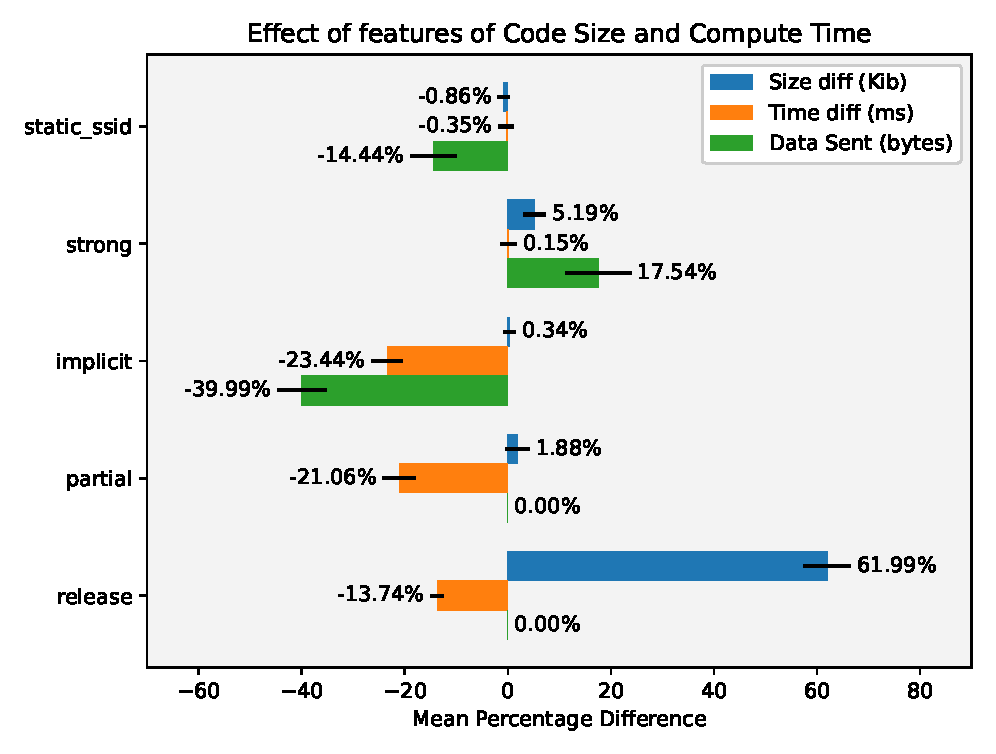
\includegraphics[width=\linewidth]{assets/feature_effects.eps}
  \caption{Plot of the effect of different feature flags and compiler modes}
  \label{fig:feature-effects}
\end{figure}

\subsection{Comparison With OPAQUE}
In order to evaluate the performance of the \gls{aucpace} implementation an implementation of an equivalent protocol to compare against is required.
\gls{opaque} is another modern \gls{apake}, it was the winner of the \gls{ietf}'s \gls{pake} selection competition, edging out \gls{aucpace} in the final round.
This makes it a perfect comparison protocol for \gls{aucpace}.
The implemention of \gls{opaque} we are going to compare against is \texttt{opaque-ke} an implementation from Whatsapp.
It was picked as it is the most downloaded version on \href{https://crates.io/}{crates.io}.
The data for \gls{opaque} can be found in \cref{tab:opaque-embedded-benchmarks}.
The mean code size for \gls{aucpace} was 85Kib in server mode and 137Kib in release mode, this is marginally less than \gls{opaque} with the difference being more significant in the release compilation mode.
Compute time is where \gls{aucpace} really shines, with even the slowest result for \gls{aucpace} (171ms) being faster than the fastest for \gls{opaque} (192ms).
On average \gls{aucpace} is $62.7\%$ faster in release mode and $62.0\%$ faster in server mode.
\gls{aucpace} stands out once again in data sent, all variants of \gls{aucpace} sent less data than \gls{opaque}, the least data-intensive \gls{aucpace} variant sent just 166 bytes, almost 3x less than \gls{opaque} on 486.
In summary \gls{aucpace} takes up less space, takes less time to compute and sends less data over the network.

\clearpage

\begin{center}
  \rowcolors{0}{}{mintbg}
  \captionof{table}{Code size and compute time by compilation profile for OPAQUE}
  \label{tab:opaque-embedded-benchmarks}
  \begin{tabular}{ cccc }
    \toprule
    profile & code size (Kib) & compute time (ms) & data sent (bytes) \\
    \midrule
    \texttt{server}  & 87 & 222 & 486 \\
    \texttt{release} & 151 & 192 & 486 \\
    \bottomrule
  \end{tabular}
\end{center}

\section{Breaking Everything}
By happenstance I was reading NCC Group's recent review of Whatsapp's \texttt{opaque-ke} crate \cite{whatsapp-are-dumb-too, whatsapp-are-dumb-too-report}.
While reading the report the following finding caught my eye:
\begin{figure}[H]
  \centering

  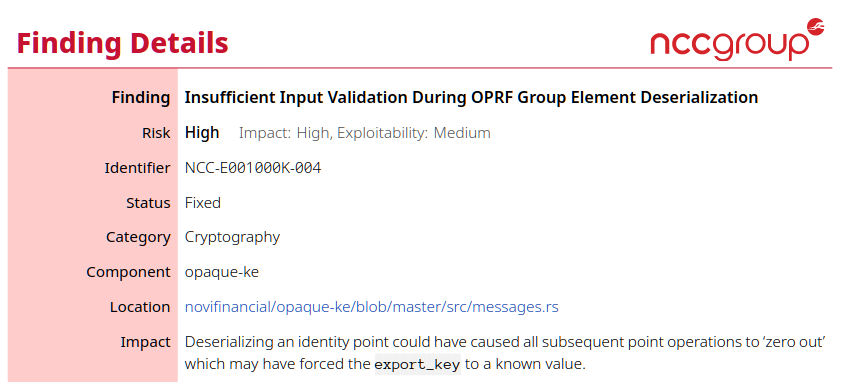
\includegraphics[width=\linewidth]{high_finding.png}
  \caption{High severity finding from \cite{whatsapp-are-dumb-too-report}.}
  \label{fig:high-severity-finding}
\end{figure}

In Whatsapp's implementation of OPAQUE \cite{opaque}, they used the \texttt{RistrettoPoint} type from \texttt{curve25519-dalek}, and while deserialising this type they didn't have any checks to see if this point was the identity point.
\Citeauthor{whatsapp-are-dumb-too-report} point out that this leads all subsequent point operations to \enquote{zero out} and thus cause the shared key to have a known value.
Unsure of whether this would also break my \gls{aucpace} implementation I modified \texttt{key\_agreement.rs} to have the client act as a malicious adversary and to send this identity point.

\rustcode{Malicious AuCPace Client}{assets/neutral_point_send.rs}

\begin{figure}[H]
  \centering

  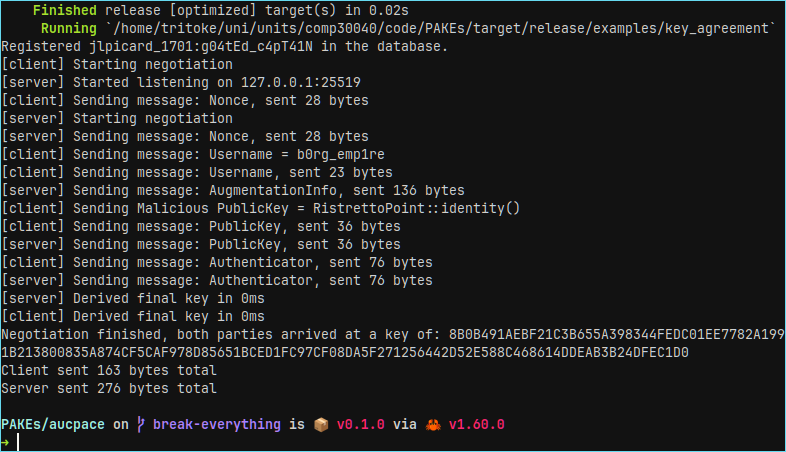
\includegraphics[width=\linewidth]{malicious_aucpace.png}
  \caption{Malicious AuCPace Client}
  \label{fig:break-everything}
\end{figure}

To my dismay it worked.
I immediately imformed RustCrypto of the problem and started working on a fix.

\subsection{Identifying the Extent of the Damage}
So what could a malicious attacker do with this bug?

\begin{itemize}
  \item{Impersonate any user, even a user who has never registered, even when no user has ever registered.}
  \item{Impersonate any server, to any user, regardless of whether they've registered with the server.}
\end{itemize}

Safe to say this is about as bad as it gets.

\subsection{Fixing the Problem}
Thankfully the fix for this issue is incredibly simple.
The \gls{aucpace} protocol specifies points at which to abort the protocol should an invalid point be encountered.
Thus everywhere \gls{aucpace} says to abort if the point is invalid, we put in a check for the identity point.

\codediff[minted options={firstline=575, lastline=589}]{Patch for checking the identity element.}{assets/fix.diff}

It is clear to see that this is a very simple patch the main issue is ensuring it is caught everywhere.

\subsection{Why Was This Not Caught Earlier?}
There are several reasons why this wasn't caught earlier:
\begin{enumerate}
  \item{My lack of familiarity with \gls{ecc} -- this was my first time ever using \gls{ecc} and it was simply not something I knew to look out for.}
  \item{My decision to implement based on the paper not the \gls{ietf} document -- the paper mentions only to abort if a point is invalid. However there are two ways a point can be invalid, it can be off the curve, and it can be the identity point. \texttt{curve25519-dalek} makes the former unrepresentable using Rust's type system, hence my belief that this check was unnecessary. However the \gls{ietf} draft of \gls{aucpace} mentions explicitly to check for the identity element \cite{ietf-aucpace}.}
  \item{This is quite a subtle bug -- it is hard to spot when you are unfamiliar with \gls{ecc}, case and point Whatsapp made this mistake as well, and so did the the core developers of Java. Java's CVE-2022-21449 \enquote{Psychic Signatures} \cite{java-psychic-signatures}, had the same bug in their implementation of \gls{ecdsa}. Introduced in commit \texttt{3c12c4b0f35} Dec 2018 fixed in \texttt{e2f8ce9c3ff} Jan 2022, all in it took 3 years for this same bug to get found and patched in Java.}
\end{enumerate}

\subsection{How To Prevent This Bug From Ever Happening Again?}
Two changes have been implemented to prevent this bug from ever happening again:
\begin{enumerate}
  \item{Every method that handles a RistrettoPoint from the network checks it to make sure it is not the identity point.}
  \item{There are now tests for every method of both the Client and Server to ensure that providing an invalid point returns an \texttt{IllegalPointError}.}
\end{enumerate}

There is a better way to fix this however, RustCrypto's \texttt{elliptic-curve} module solves this problem using the power of Rust's type system.
They have a \texttt{NonIdentity} type which is guaranteed to never be the identity element.
When Curve25519 is introduced to \texttt{elliptic-curve} the library will be refactored to move over to this type.

